\documentclass{article}
\usepackage{listings}
\usepackage[utf8]{inputenc}
\usepackage{ amssymb }
\usepackage{amsfonts}
\usepackage{graphicx}

\title{Sistemas Distribuidos y Verificación \\ Tarea 2}
\author{Fabián Romero Jiménez}
\begin{document}
\maketitle

\begin{enumerate}

\item[\bf{Problema 1}] Considera el modelo de memoria compartida visto en clase libre de espera, y el diagrama de la Figura 1. Donde las flechas indican la especificación de la tarea $\delta$.\\

\begin{center}
  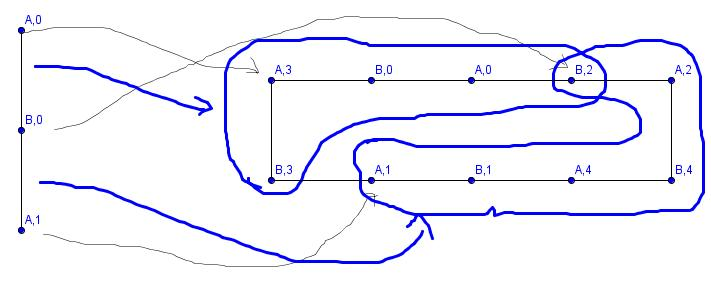
\includegraphics{t2_f1.png}\\
  Figura 1
\end{center}

\begin{enumerate}

\item Demuestra que existe un protocolo que puede resolver la tarea, considera que se puede ejecutar más de una lectura y escritura sobre el mismo arreglo mem[A,B].

\item Demuestra que con un protocolo de una ronda no se puede resolver
el problema.

\end{enumerate}

\item[\bf{Problema 2}] Sea $\delta$ un mapeo simplicial, que nos lleva de una gráfica $G$ a una gráfica $H$, $\delta$ mapea los vértices de G sobre todos los vértices de H.

Demuestra que si G es conexo entonces H es conexo.
Demuestra que si $\delta$ preserva colores entonces es rigido, es decir, mapea
vértices diferentes a vértices diferentes.

\item[\bf{Problema 2}] Sea $\delta$ un mapeo simplicial, que nos lleva de una gráfica $G$ a una gráfica $H$, $\delta$ mapea los vértices de G sobre todos los vértices de H.

\end{enumerate}
\end{document}
